Lensing pipelines are not able to return 
a shear measurement for all galaxies in an
image. If a lensing pipelines preferentially rejects 
objects then the assumption that the population of galaxies used to
measure shear have $< \epsilon > = 0 $ may no longer be true. 
This selection bias effect has been discussed in STEP1 
where it was determined that results for some lensing pipelines  
improved when the non-zero mean intrinsic ellipticity of the surviving 
objects was corrected for. \\
\indent The fraction of successful shear measurements
 for each pipeline is shown for sources SNR $>$ 20 in Table \ref{table:sur_sel}.
The pipelines with the highest efficiency of successful measurements
are PK, DE and KM which are all moment based methods. 
As implemented in this challege the GM method
rejects a portion of the returned shear measurements and 
uses a weighting system in determining the average shear. Before the
flagged objects were rejected, the efficiency of GM was 0.93 and after
the efficiency was 0.24. The efficency of GM reported here is
therefore not directly comparable to the other lensing pipelines. 
\\
\indent
Pipelines may reject objects in a ellipticity dependent way. To test
for this selection effect bias, the $\gamma$ measured is corrected for
the intrinsic ellipticity of the sources as measured by each lensing
pipeline. I3 and DE do not appear to have a selection bias as their
accuracy is similar, before and after correction for $< \epsilon > \neq 0 $. The
pipeline that is most affected by selection bias is PF. Q, M and C as measured for each
lensing pipeline after correcting for selection effects is included in
Table \ref{table:QMC_sel} and Table \ref{table:MC_sel} . 
%%%%%%%%%%%%%%%%%% ************************
\begin{table}
        \centering
        \begin{tabular}{|c|c|c|c|c|c|c|c|}  
          \hline
          Pipeline  &  efficiency \\
          \hline
          DE &  0.92 \\
          \hline
          PF & 0.86 \\
          \hline
          GM & 0.24 (0.93) \\
          \hline
          MJ & 0.81 \\
          \hline
          PK & 0.90 \\
          \hline
          I3 &  0.79 \\
          \hline
          IM &  0.55 \\
          \hline
          KM & 0.91 \\
          \hline
        \end{tabular}
        \caption{The percentage survival of the shape measurement pipelines.}
    \label{table:sur_sel}
\end{table}



\begin{figure}
\centering
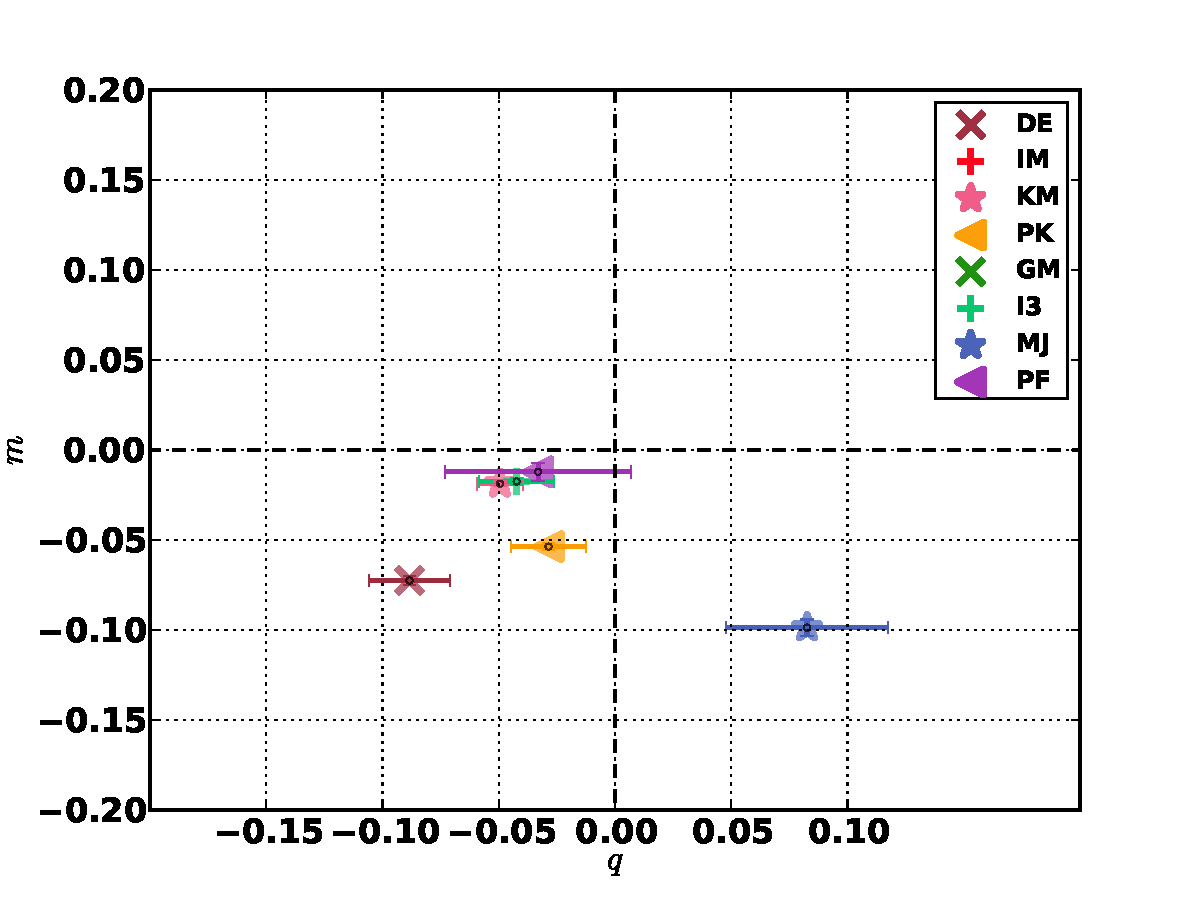
\includegraphics[width=0.5\textwidth]{fig/QMC_main_sel_f.pdf} \\
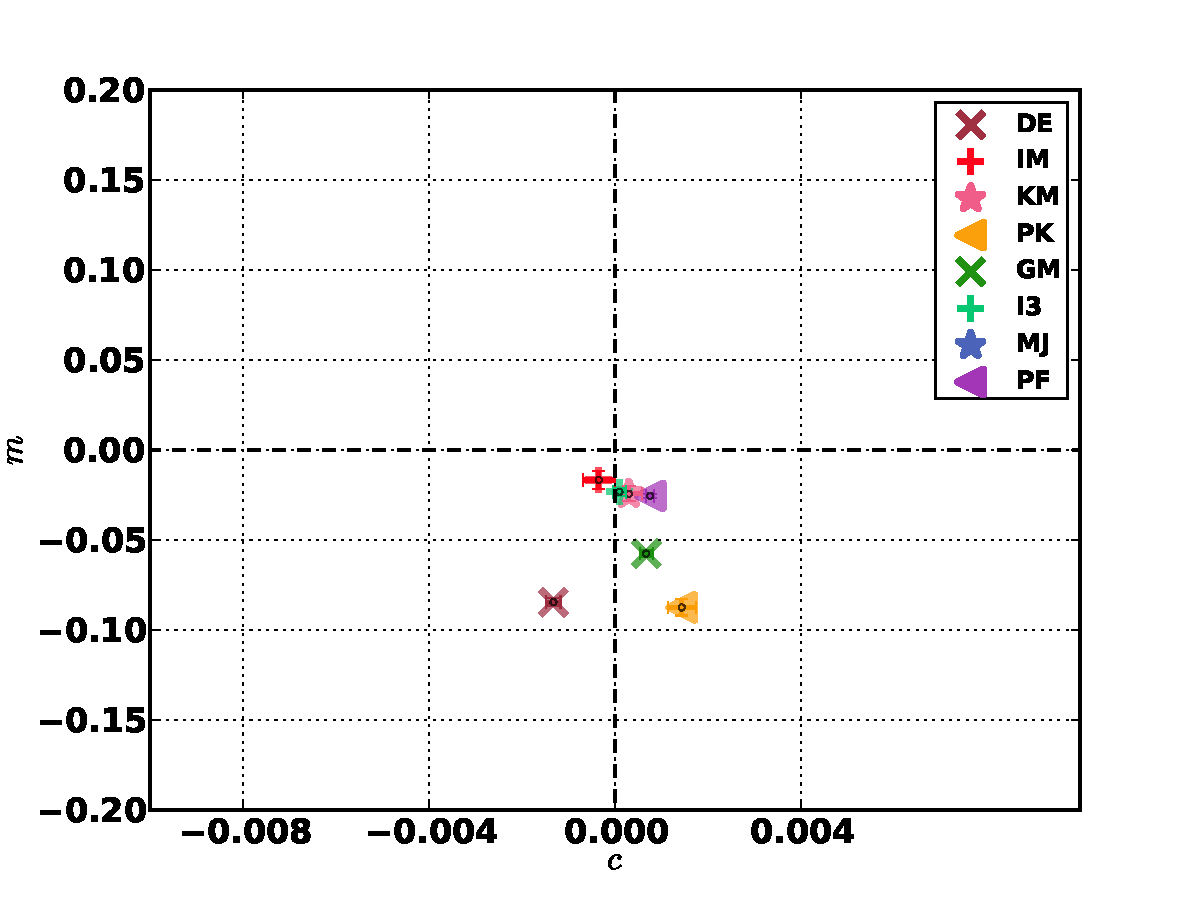
\includegraphics[width=0.5\textwidth]{fig/MC_main_sel_f.pdf} 
\caption{Average Q and M results for all pipelines for objects 
SNR $>$ 20 after correcting for selection effects in the top
panel and average M and C results for all pipelines
for objects SNR $>$ 20 in the bottom panel.}
\label{fig:QMC_main_sel}
\end{figure}

